\section{Coordination}\label{coordination}
This section analyses the messages exchanged between the entities composing the prototype architecture. There are three phases in this coordination process:
\begin{enumerate}
    \item \textbf{Grid connection}
    \item \textbf{Recruitment}
    \item \textbf{P2P messaging}
\end{enumerate}

\subsection{Grid connection}
This phase connects a Node (whether used by the Mobile or Desktop client) or an Invoking Endpoint Prototype to the Broker Service using a Socket connection through the Socket.io framework. The Broker Service registers the connections and uses them in the Recruitment phase.

\subsection{Recruitment}
The recruitment phase connects a requestor device (that becomes the Master in the P2Pconnection) to an actual device that will perform a Contribution (becoming the Slave). While a Slave is necessarily a Node, a Master can either be an Invoking Endpoint or a Node, allowing to obtain both Invoking Endpoint to Node connections and Node to Node connections.

This phase is executed exchanging messages between the soon-to-be Peers using the previously established Socket connections, but ends with a direct P2P connection between the Master and the Slave through the WebRTC framework.

\vspace{4mm}

\begin{figure}[!ht]
    \centering
    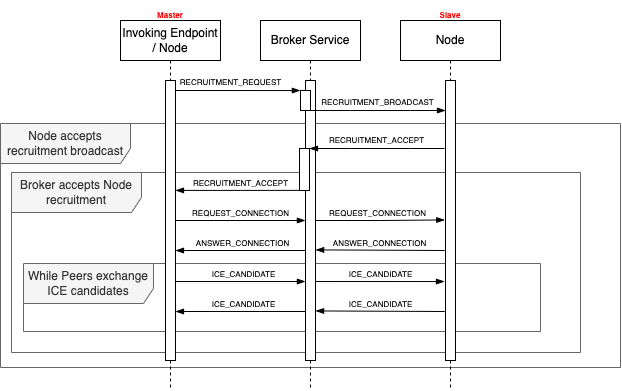
\includegraphics[width=\linewidth]{document/chapters/chapter_7/images/recruitment_messages.png}
    \caption{Recruitment - Sequence Diagram}
    \label{fig:recruitment_messages}
\end{figure}

\textit{Figure \ref{fig:recruitment_messages}} shows the actual messages exchanged in this phase: the soon-to-be Master sends a RECRUITMENT\_REQUEST to the Broker Service, containing details for which kind of resources are needed; the Broker Service, upon receiving this request, creates a pending Recruitment Request and broadcasts a RECRUITMENT\_REQUEST message to all the connected Nodes.

The Node checks locally if it is compatible with the received request and, if all the conditions are true, it sends a RECRUITMENT\_ACCEPT message to the Broker Service which, upon receiving it, checks if the request is still unsatisfied, eventually forwarding the message to the entity that first emitted the request.

\subsection{P2P messaging}
TODO
\begin{figure}[!ht]
    \centering
    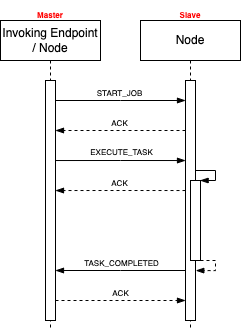
\includegraphics[scale=0.8]{document/chapters/chapter_7/images/p2p_messages.png}
    \caption{P2P messaging - Sequence Diagram}
    \label{fig:p2p_messages}
\end{figure}